\documentclass[10pt,letterpaper,onecolumn,fontset=none]{ctexart} %article ctexart
%\usepackage[a4paper]{geometry}
%\usepackage{indentfirst}   %用于首行自动缩进的宏包
\usepackage{lipsum}   %随机生成文本
\usepackage{subfigure}   
\usepackage{float}   
\usepackage{amsmath,amsfonts,amsmath,amsthm} %美国数学协会宏包
\usepackage{bm} %bold math
\usepackage{xcolor}
\usepackage{graphicx}  %插入jpg图片
\usepackage{tikz} %插入tikz图片
\usetikzlibrary{shapes,arrows,chains} %
\usepackage{booktabs}
\usepackage{enumitem} %enumrate
\usepackage{tabularx} %弹性列表格
\usepackage{multido} %loop do
\usepackage{ulem} %强调文本,例如\uline

% \usepackage[style=numeric,
%             sorting=none,
%             bibstyle=gb7714-2015,
% 			  citestyle=gb7714-2015]{biblatex} %biblatex
\usepackage[bibstyle=numeric,
			gbpub=false,
            sorting=none,
            style=gb7714-2015,
            citestyle=gb7714-2015]{biblatex} %biblatex
\usetikzlibrary{arrows,shapes,chains} 


% font set
\setCJKmainfont{FangSong}[AutoFakeBold]
%上述包报警告:Some font shapes were not available.
%或 Font shape 'TU/Fangsong(0)/bx/n' undefined
%指 FangSong字体无粗体,ctex将使用伪粗体替代
\setmainfont{Times New Roman}

\newfontfamily\FangSong{FangSong}
\newfontfamily\NewRoman{Times New Roman}

% path set
\graphicspath{./}
\bibliography{./ref.bib}

% pagestyle
\pagestyle{plain}

% personal information
\title{Latex Template}
\author{variant}
\date{\today}

% 引理
\newtheorem{lemma}{Lemma}[subsection]

% 正文
\linespread{1.5}
\begin{document}

\newpage
\thispagestyle{empty} %本页页面样式: 无页眉页脚页码等
\vskip 2cm
\begin{figure}[htpb]	\centering
	
\includegraphics[width=0.95\textwidth]{fig/ZJU.png}
\end{figure}
\begin{figure}[htpb]	\centering
	
\includegraphics[width=0.5\textwidth]{fig/ZJUlogo.png}
\end{figure}

\begin{center}
	\bfseries
	\zihao{4}
	\begin{tabularx}{.8\textwidth}{>{\FangSong}l >{\NewRoman}X<{\centering}}
		题目        &  \uline{Latex Template} \\
		~          &  ~\\
		学生姓名    & \uline{\hfill variant \hfill} \\
		学生学号    & \uline{\hfill 147258369 \hfill} \\
		年级与专业  & \uline{\hfill \mbox{20}ISEE \hfill} \\
		~          & ~\\
		递交日期    &  \uline{\hfill \today \hfill} \\
	\end{tabularx}
\end{center}


\newpage
\tableofcontents %TOC
\thispagestyle{empty}
\newpage

\pagenumbering{arabic} %页码起始处
\maketitle %显示标题
\begin{abstract}
	\lipsum[3]
\end{abstract}
\noindent \textbf{Keywords: } apple, applepen, pineapplepen

% 大节
\section{Section 1}
\lipsum[17] %随机生成一段文字
% 小节
\subsection{subsection 1.1}
\lipsum[16]
\begin{enumerate}[itemindent=0pt,topsep=0pt,leftmargin=*,parsep=0pt,itemsep=0pt,label=(\arabic*)]
	\item \lipsum[2]
	\item \lipsum[2]
	\item \lipsum[3]
\end{enumerate}

% 小节
\subsection{subsection 1.2}
\lipsum[11] %随机生成一段文字
As shown in Figure~\ref{fig1}.

%图表
\begin{figure}[H]
	\centering
	\subfigure[Harr feature]{
		\label{fig:a} 
		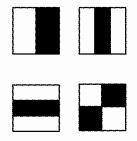
\includegraphics[width=2cm,height=2cm]{fig/1.jpg}}
	\vfill
	\subfigure[Integrogram]{
		\label{fig:subfig:b} 
		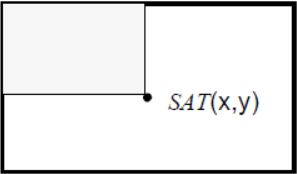
\includegraphics[width=2cm,height=1.8cm]{fig/2.jpg}}
	\qquad
	\subfigure[Calculate]{
		\label{fig:subfig:c} 
		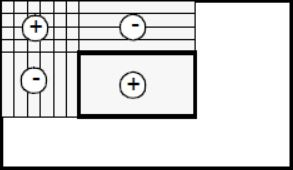
\includegraphics[width=2cm,height=1.8cm]{fig/3.jpg}}
	\caption{Schematic Diagram} %caption必须在label前以确保被ref检索
	\label{fig1} 
\end{figure}

% 小节
\subsection{subsection 1.3}
\lipsum[22]
\begin{lemma} \label{Kexist}
    If a kernel matrix $K$ can be written as $K=\tilde{K}+\epsilon I$ , where $\epsilon > 0,\quad \tilde{K} \succeq 0$ and $I$ is the identity matrix, then the kernel function corresponding to $K$ is universal\cite{zjugradthesisrules}.
\end{lemma}
\lipsum[5]   %随机生成一段文字
\par the formula is as follows\ref{eq:softquant}:

% 公式
\begin{equation} \label{eq:softquant}
\tilde{z}_i = \sum_{j=1}^L \frac{\exp(-\sigma\|z_i-c_j\|)}{\sum_{l=1}^L \exp(-\sigma\|z_i-c_l\|)} c_j
\end{equation}

\begin{eqnarray} \label{eq:case1}
	c(\psi) = 
	\begin{cases}
	  2H(\psi-1)-2(\psi-1)/n   & \psi>2\\
	  1                        & \psi=2\\
	  0                        & \psi<2  
	\end{cases}
\end{eqnarray}

\begin{equation} \label{eq:case2}
	\begin{split}
	  &min_\mathbf{\alpha}\frac{1}{2}\sum_{ij}\alpha_i\alpha_j k(\mathbf{x_i},\mathbf{x_j}) \\
	  &subject\ to\ 0 \leq \alpha_i \leq \frac{1}{v\ell},\ \sum_{i}^{}\alpha_i=1
	\end{split}
\end{equation}

% 大节
\section{Section 2}

% 小节
\subsection{subsection 2.1}
\lipsum[2]   %随机生成一段文字
The flow chart is shown below\cite{zjuthesisrules}:

%流程图
\begin{figure}[H]
	\centering
	\scriptsize %同上标字体
	\tikzstyle{format}=[rectangle,draw,thin,fill=white,align=center]
	\tikzstyle{point}=[coordinate,on grid,]
	\begin{tikzpicture}[node distance=20mm,
	auto,>=latex',thin,start chain=going right,every join/.style={norm},]
	\node[point] (n0){PA};
	\node[format,right of=n0,node distance=17mm,] (n1){RGB to\\AXI-Stream};
	\node[format,right of=n1,node distance=20mm,] (n2){Image\\Processing};
	\node[format,right of=n2,node distance=17mm,] (n3){VDMA};
	\node[format,right of=n3,node distance=15mm,] (n4){DDR3};
	\node[format,right of=n4,node distance=14mm,] (n5){DDR3};	
	\draw[->] (n0.east) to node {Input} (n1);
	\draw[->] (n1.east) -- (n2);
	\draw[->] (n2.east) -- (n3);
	\draw[<->] (n3.east) to node {} (n4);
	\draw[<->] (n4.east) to node {} (n5);
	\end{tikzpicture}
	\caption{Flow Diagram}
	\label{fig2} %label置于caption后
\end{figure}


% Define block styles
	
\begin{figure}[]
	\centering
	\tikzstyle{decision} = [diamond, draw, fill=blue!20, 
    text width=4.5em, text badly centered, node distance=3cm, inner sep=0pt]
	\tikzstyle{block} = [rectangle, draw, fill=blue!20, 
    text width=5em, text centered, rounded corners, minimum height=4em]
	\tikzstyle{line} = [draw, -latex']
	\tikzstyle{cloud} = [draw, ellipse, fill=red!20, node distance=3cm,
    minimum height=2em]
	\begin{tikzpicture}[node distance = 2cm, auto]
		% Place nodes
		\node [block] (init) {initialize model};
		\node [cloud, left of=init] (expert) {expert};
		\node [cloud, right of=init] (system) {system};
		\node [block, below of=init] (identify) {identify candidate models};
		\node [block, below of=identify] (evaluate) {evaluate candidate models};
		\node [block, left of=evaluate, node distance=3cm] (update) {update model};
		\node [decision, below of=evaluate] (decide) {is best candidate better?};
		\node [block, below of=decide, node distance=3cm] (stop) {stop};
		% Draw edges
		\path [line] (init) -- (identify);  
		\path [line] (identify) -- (evaluate);
		\path [line] (evaluate) -- (decide);
		\path [line] (decide) -| node [near start] {yes} (update); % "-|" 指折线,横竖
		\path [line] (update) |- (identify);
		\path [line] (decide) -- node {no}(stop); 
		\path [line,dashed] (expert) -- (init);
		\path [line,dashed] (system) -- (init);
		\path [line,dashed] (system) |- (evaluate);
	\end{tikzpicture}
	\caption{Flow Diagram2}
	\label{fig3} %label置于caption后
\end{figure}

\begin{figure}[]
	\centering
	\scriptsize
	\tikzstyle{decision} = [diamond, draw, fill=blue!20, 
    text width=4.5em, text badly centered, node distance=3cm, inner sep=0pt]
	\tikzstyle{block} = [rectangle, draw, fill=blue!20, 
    text width=5em, text centered, rounded corners, minimum height=4em]
	\tikzstyle{line} = [draw, -latex']
	\tikzstyle{cloud} = [draw, ellipse, fill=red!20, node distance=3cm,
    minimum height=2em]
	% \begin{tikzpicture}[node distance = 2cm, auto]
	% 	\node [block] (P) {某行业}
	% \end{tikzpicture}
\end{figure}


% 小节
\subsection{subsection 2.2}
\lipsum[11]   %随机生成一段文字
The table is shown below:
\begin{table}[H]
	\centering
	\caption{Three Wire Table}
	\label{fig4}
	\begin{tabular}{cccc}
		\toprule
		&PC(ms) &arm(ms) &fpga(ms)\\
		\midrule
		Open &100 &176 &322\\
		Close &223 &967 &178\\
		\bottomrule	
	\end{tabular}
\end{table}

\mbox{} \vfill
\begin{flushright}
	\bfseries \zihao{-4}
	指导教师(签名) \underline{\multido{}{5}{\quad}} 职称 \underline{\multido{}{5}{\quad}}
\end{flushright}

\newpage

\printbibliography

\end{document}